\section{Bayarjavkhlan Byambadorj}
\label{sec:Maks}

\subsection{Równanie kwadratowe}

    \textbf{Równanie kwadratowe} równanie algebraiczne z jedna niewiadoma w drugiej potedze i opcjonalnie niższych. Innymi słowy równanie wielomianowe drugiego stopnia, czyli równanie postaci: \[ax^{2}+bx+c = 0\]
    Gdzie: $a,b,c$ sa jego współczynnikami rzeczywistymi, zespolonymi badź sa elementami dowolnego ciała. Zakłada sie, że \(a\neq0\) dzieki czemu równanie nie degeneruje sie do równania liniowego. Współczynniki niekiedy nazywane sa kolejno: kwadratowym, liniowym i stałym (badź wyrazem wolnym).Inna nazwa równania kwadratowego jest równanie drugiego stopnia.

\subsection{Wykres funkcji}

    \begin{figure}[h]
        \centering
        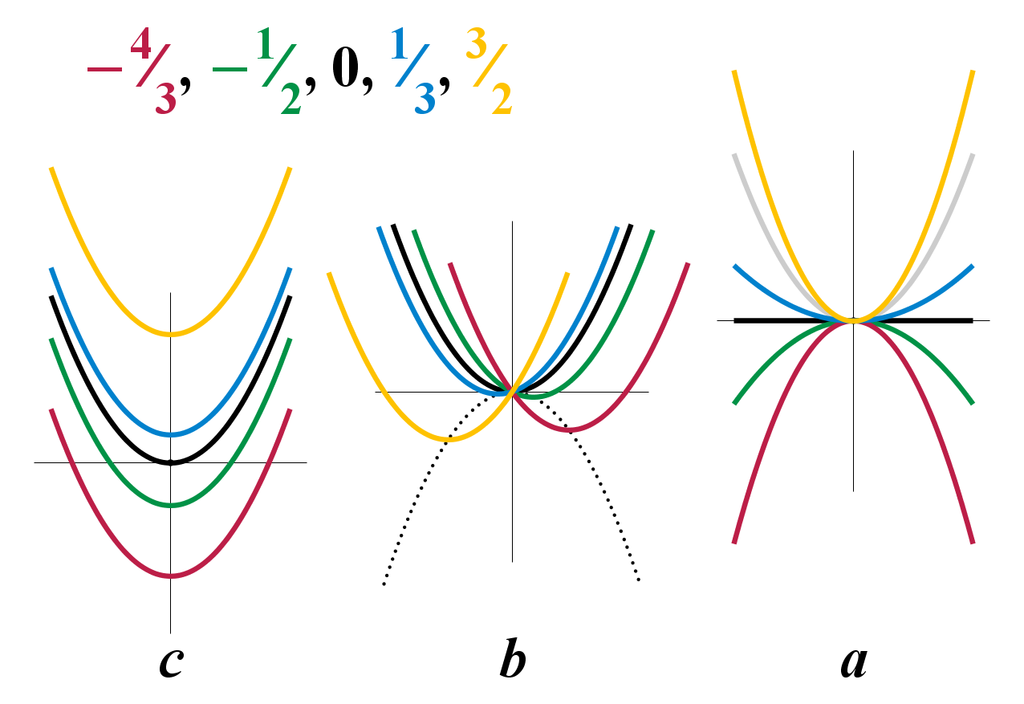
\includegraphics[width=0.75\textwidth]{pictures/Quadratic_equation_coefficients.png}
        \caption{Wykres funkcji kwadratowej zmiennej rzeczywistej przy zmianie różnych współczynników}
        \label{fig:mesh1}
    \end{figure}
    
\newpage
\subsection{Rozwiazanie}

    Równanie kwadratowe, które można rozwiazać za pomoca tego wzoru:
    \[x_{1,2} = -b - \frac{\sqrt{b^{2} - 4ac}}{2a}\]
    
    Stad: 
    
    \[ \delta = \sqrt{b^{2} - 4ac}\]

    \begin{enumerate}
            \item ($\Delta$ > 0), to równanie ma dwa rozwiazania rzeczywiste (dwa pierwiastki rzeczywiste)
            \item ($\Delta$ = 0), to równanie ma jedno rozwiazanie rzeczywiste (podwójny pierwiastek rzeczywisty),
            \item ($\Delta$ < 0), to równanie nie ma rozwiazań rzeczywistych.
        \end{enumerate}

\subsection{Listy}
        \begin{enumerate}
            \item Pierwszy numerowany element
            \item Drugi numerowany element
            \begin{enumerate}
                \item zagniezdzony element
            \end{enumerate}
        \end{enumerate}
    \subsubsection{Lista nienumerowana}
        \begin{itemize}
            \item Pierwszy element
            \item Drugi element
            \begin{itemize}
                \item zagniezdzony element
            \end{itemize}
        \end{itemize}
\subsection{Krotki tekst}
    To jest pierwszy akapit, jest on \textbf{pogrubiony} oraz \textit{pochylony} \\
    \underline{Natomiast w drugim akapicie wszystko jest podkreslone}